\section{图遍历}
图是表示实体之间关系的数据结构。 涉及的实体表示为顶点,关系表示为边。 
许多重要的现实世界问题自然地被表述为大规模图问题,并且可以从大规模并行计算中受益。 突出的例子包括社交网络和行车路线图服务。 
并行化图计算有多种策略,其中一些以并行处理顶点为中心,而另一些则以并行处理边为中心。 图本质上与稀疏矩阵相关。 
因此,图计算也可以用稀疏矩阵运算来表示。 然而,人们通常可以通过利用特定于所执行的图计算类型的属性来提高图计算的效率。 
在本章中,我们将重点讨论图搜索,这是许多现实世界应用程序的基础的图计算。

\subsection{背景}
图数据结构表示实体之间的关系。 例如,在社交媒体中,实体是用户,关系是用户之间的联系。 
又例如,在行车路线图服务中,实体是位置,关系是位置之间的道路。 有些关系是双向的,例如社交网络中的朋友关系。 
其他关系是定向的,例如道路网络中的单向街道。 在本章中,我们将重点关注方向关系。 
双向关系可以用两个方向关系来表示,每个方向一个。

\begin{figure}[H]
	\centering
	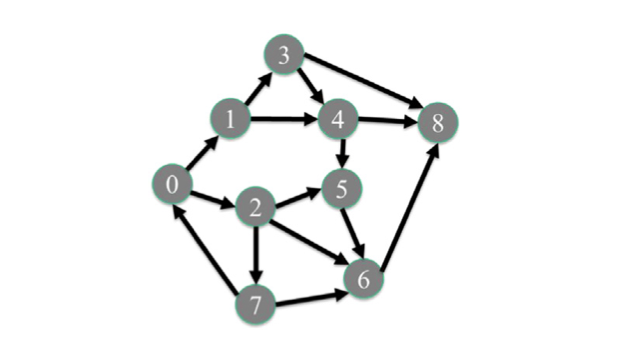
\includegraphics[width=0.9\textwidth]{figs/F15.1.png}
	\caption{\textit{具有 9 个顶点和 15 个有向边的简单图示例。}}
\end{figure}

图 15.1 显示了带有方向边的简单图的示例。 方向关系表示为从源顶点到目标顶点的带箭头的边。 
我们为每个顶点分配一个唯一的编号,也称为顶点 $i d$。 有一条边从顶点 0 到顶点 1 ,一条边从顶点 0 到顶点 2 ,依此类推。

图的直观表示是邻接矩阵。 如果存在从源顶点 $i$ 到目标顶点 $j$ 的边,则邻接矩阵的元素 $\mathrm{A}[i][j]$ 的值为 1 。 
否则,它是 0 。 图 15.2 显示了图 15.1 中简单图的邻接矩阵。 
我们看到 $A[1][3]$ 和 $A[4][5]$ 是 1 ,因为存在从顶点 1 到顶点 3 的边。 为了清楚起见,我们将 0 值保留在邻接矩阵之外。 
也就是说,如果一个元素为空,则其值被理解为 0 。

\begin{figure}[H]
	\centering
	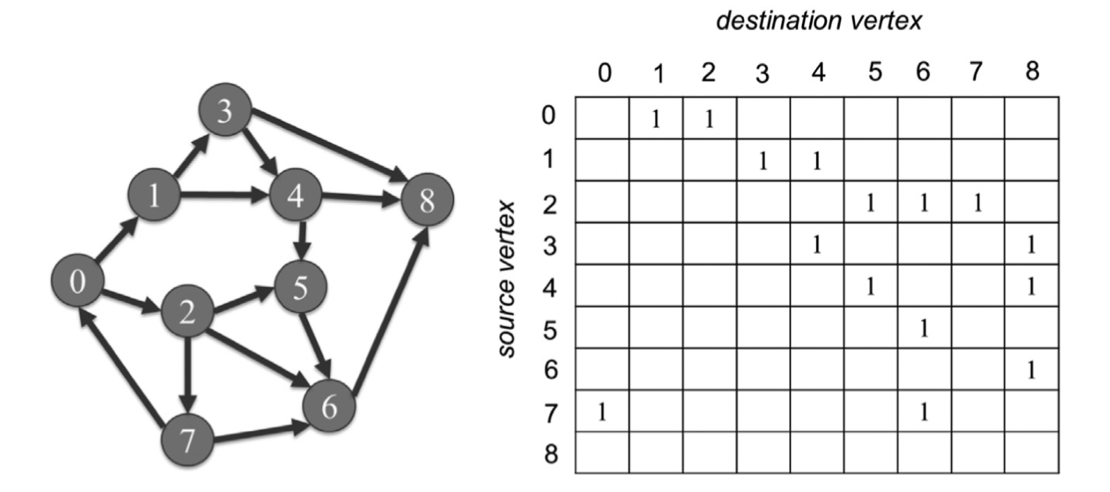
\includegraphics[width=0.9\textwidth]{figs/F15.2.png}
	\caption{\textit{简单图示例的邻接矩阵表示。}}
\end{figure}

如果具有 $\mathrm{N}$ 个顶点的图是全连接的,即每个顶点都与所有其他顶点连接,则每个顶点应该有 $(\mathrm{N}-1)$ 出边。 
总共应该有 $\mathrm{N}(\mathrm{N}-1)$ 边,因为没有从顶点到自身的边。 
例如,如果我们的九顶点图是完全连接的,则每个顶点应该有八条边。 总共应该有 72 条边。 
显然,我们的图的连通性要差得多; 每个顶点具有三个或更少的出边。 这样的图被称为稀疏连接图。 
也就是说,每个顶点的平均出边数远小于$\mathrm{N}-1$。

此时,读者很可能已经做出了正确的观察,稀疏连接的图可能会受益于稀疏矩阵表示。 
正如我们在第 14 章“稀疏矩阵计算”中所看到的,使用矩阵的压缩表示可以大大减少所需的存储量和零元素上浪费的操作数量。 
事实上,许多现实世界的图都是稀疏连接的。 
例如,在 Facebook、Twitter 或 LinkedIn 等社交网络中,每个用户的平均连接数远小于用户总数。 
这使得邻接矩阵中非零元素的数量远小于元素总数。

\begin{figure}[H]
	\centering
	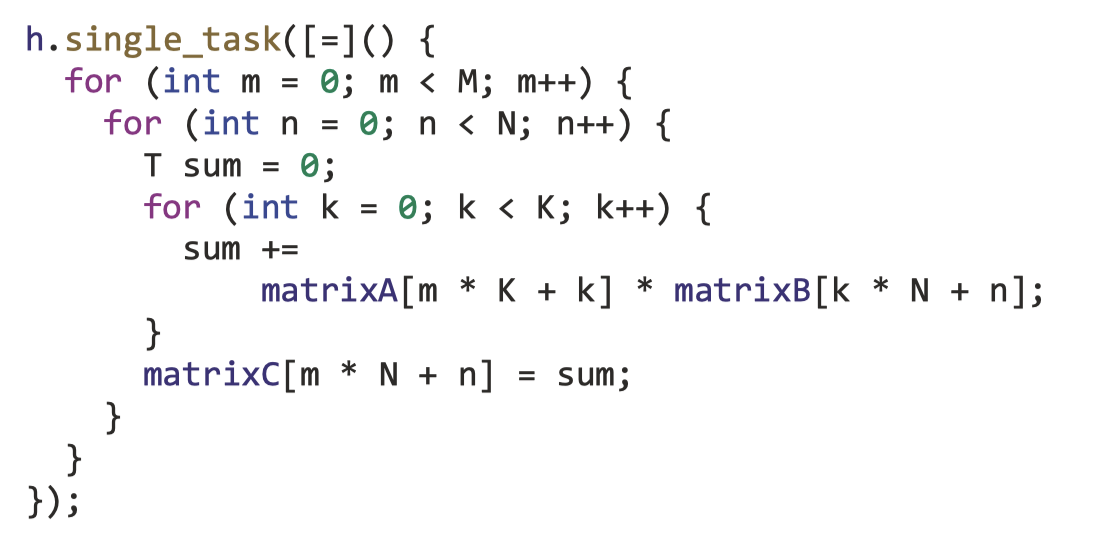
\includegraphics[width=0.9\textwidth]{figs/F15.3.png}
	\caption{\textit{邻接矩阵的三个稀疏矩阵表示:(A) CSR、(B) CSC、(C) COO, 
	COO 坐标; CSC,压缩稀疏列; CSR,压缩稀疏行。}}
\end{figure}

图 15.3 显示了使用三种不同存储格式的简单图示例的三种表示形式:压缩稀疏行(CSR)、压缩稀疏列(CSC)和坐标(COO)。 
我们将行索引和指针数组分别称为 src 和 srcPtrs 数组,将列索引和指针数组分别称为 dst 和 dstPtrs 数组。 
如果我们以 CSR 为例,请回想一下,在稀疏矩阵的 CSR 表示中,每个行指针给出了行中非零元素的起始位置。 
类似地,在图的 CSR 表示中,每个源顶点指针 (srcPtrs) 给出顶点出边的起始位置。 
例如,srcPtrs [3]=7 给出原始邻接矩阵第 3 行中非零元素的起始位置。 
此外,srcptrs $[4]=9$ 给出原始矩阵第 4 行中非零元素的起始位置。 
因此,我们期望在 data[7] 和 data[8] 中找到第 3 行的非零数据,
以及在 dst[7] 和 dst[8] 中找到这些元素的列索引(目标顶点)。 这些是离开顶点 3 的两条边的数据和列索引。 
我们将列索引数组称为 dst 的原因是邻接矩阵中元素的列索引给出了所表示边的目标顶点。 
在我们的示例中,我们看到源顶点 3 的两条边的目的地是 $d s t[7]=4$ 和 $d s t[8]=8$。 
我们将其作为练习留给读者,让他们对 CSC 和 COO 的表示进行类似的类比。

请注意,此示例中的数据数组是不必要的。 由于它的所有元素的值都是 1 ,所以我们不需要存储它。 
我们可以使数据隐式化,也就是说,每当存在非零元素时,我们就可以假设它是 1 。 
例如,CSR 表示的目标数组中每个列索引的存在意味着存在一条边。 
然而,在某些应用中,邻接矩阵可以存储有关关系的附加信息,例如两个位置之间的距离或两个社交网络用户建立连接的日期。 
在这些应用程序中,数据数组需要显式存储。

稀疏表示可以显着节省邻接矩阵的存储成本。 
对于我们的示例,假设可以消除数据数组,则 CSR 表示需要存储 25 个位置,而如果我们存储整个邻接矩阵,
则需要 $9^{2}=81$ 个位置。 对于现实生活中的问题,其中一小部分邻接矩阵元素非零,节省的空间可能是巨大的。 
不同的图可能具有截然不同的结构。 表征这些结构的一种方法是查看连接到每个顶点的边数的分布(顶点度)。 
以图表示的道路网络将具有相对均匀的度数分布,每个顶点的平均度数较低,因为每个道路交叉口(顶点)通常只有少量的道路与其连接。 
另一方面,Twitter 关注者图(其中每个传入边代表一个“关注”)将具有更广泛的顶点度数分布,
其中度数较大的顶点代表受欢迎的 Twitter 用户。 图的结构可能会影响实现特定图应用程序的算法的选择。

回想一下第 14 章“稀疏矩阵计算”,每个稀疏矩阵表示都为表示的数据提供了不同的可访问性。 
因此,选择用于图的表示形式会影响图遍历算法可以轻松访问有关图的哪些信息。 CSR 表示可以轻松访问给定顶点的传出边。 
CSC 表示可以轻松访问给定顶点的传入边。 $\mathrm{COO}$ 表示可以轻松访问给定边的源顶点和目标顶点。 
因此,图表示的选择与图遍历算法的选择密切相关。 
我们在本章中通过检查广度优先搜索(一种广泛使用的图搜索计算)的不同并行实现来演示这个概念。

\subsection{广度优先搜索}
一个重要的图计算是广度优先搜索(BFS)。 BFS 通常用于发现从图的一个顶点到另一个顶点所需遍历的最短边数。 
在图 15.1 的图示例中,我们可能需要找到从顶点 0 表示的位置到顶点 5 表示的位置可以采取的所有替代路线。 
通过目视检查,我们发现存在三种可能的路径:$0 \rightarrow 1 \rightarrow 3 \rightarrow 4 \rightarrow 5,0 \rightarrow 1 \rightarrow 4 \rightarrow 5$,和 $0 \rightarrow 2 \rightarrow 5$,
其中 $0 \rightarrow 2 \rightarrow 5$ 是最短的。 有多种方法可以总结 BFS 遍历的结果。 
一种方法是,给定一个称为根的顶点,用从根到该顶点所需遍历的最少边数来标记每个顶点。

\begin{figure}[H]
	\centering
	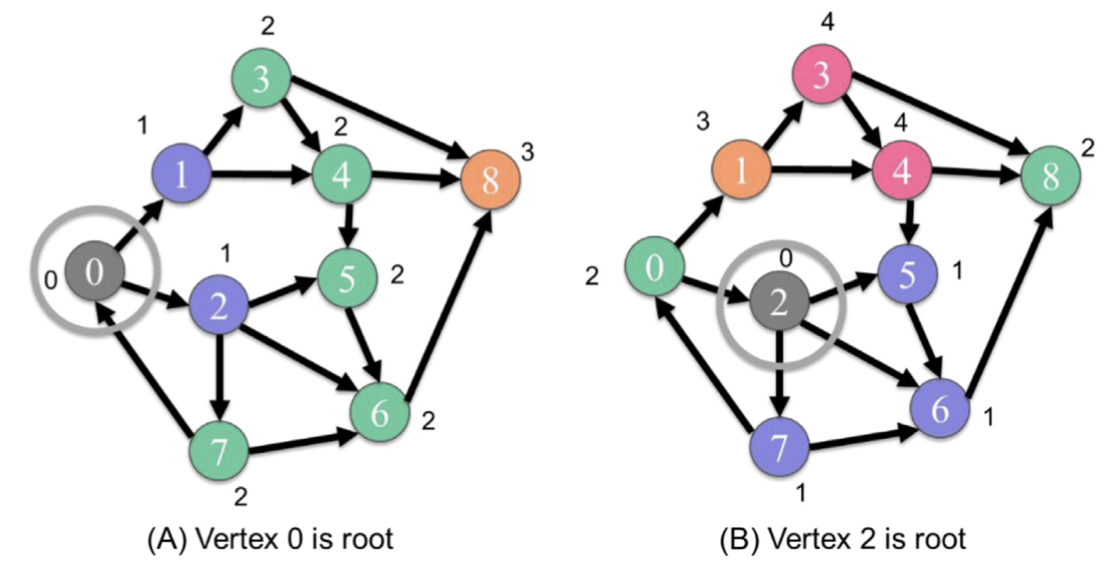
\includegraphics[width=0.9\textwidth]{figs/F15.4.png}
	\caption{\textit{(A 和 B)两个不同根顶点的广度优先搜索结果的两个示例。 
	与每个顶点相邻的标签指示从根顶点开始的跳数(深度)。}}
\end{figure}

图15.4(A)显示了以顶点0为根的期望的BFS结果。 通过一条边,我们可以到达顶点 1 和 2。
因此,我们将这些顶点标记为属于级别 1。
通过遍历另一条边,我们可以到达顶点 3(通过顶点 1)、4(通过顶点 1)、5( 通过顶点 2)、6(通过顶点 2)和 7(通过顶点 2)。 
因此,我们将这些顶点标记为属于级别 2。最后,通过再遍历一条边,我们可以到达顶点 8(通过顶点 3,4 或 6 中的任何一个)。

如果以另一个顶点为根,BFS 结果会完全不同。 图15.4(B)显示了以顶点2为根的BFS的期望结果。 
1 级顶点为 5、6 和 7。2 级顶点为 8(到顶点 6)和 0(到顶点 7)。 只有顶点 1 位于级别 3(通过顶点 0)。 
最后,4 级顶点是 3 和 4(均通过顶点 1)。 有趣的是,即使我们将根移动到距原始根仅一条边的顶点,每个顶点的结果也有很大不同。

人们可以将 BFS 的标记操作视为构建一棵以搜索的根节点为根的 BFS 树。 
该树由所有标记的顶点和仅在搜索过程中遍历的从一个级别的顶点到下一个级别的顶点的边组成。

一旦我们用级别标记了所有顶点,我们就可以轻松找到从根顶点到任何顶点的路径,其中所经过的边数等于级别。 
例如,在图15.4(B)中,我们看到顶点1被标记为级别3,因此我们知道根(顶点2)和顶点1之间的边的最小数量是3。 
如果我们需要找到路径,我们可以简单地从目标顶点开始追溯到根。 在每一步中,我们选择级别比当前顶点低一级的前驱节点。 
如果有多个相同等级的前辈,我们可以随机挑选一个。 这样选择的任何顶点都会给出一个合理的解决方案。 
事实上,有多个前辈可供选择,这意味着该问题有多个同样好的解决方案。 
在我们的示例中,我们可以通过从顶点 1 开始,选择顶点 0 ,然后选择顶点 7 ,然后选择顶点 2 ,
找到从顶点 2 到顶点 1 的最短路径。 因此,解决方案路径为 $2 \rightarrow 7 \rightarrow 0 \rightarrow 1$。 
当然,这假设每个顶点都有所有传入边的源顶点的列表,以便可以找到给定顶点的前趋。

\begin{figure}[H]
	\centering
	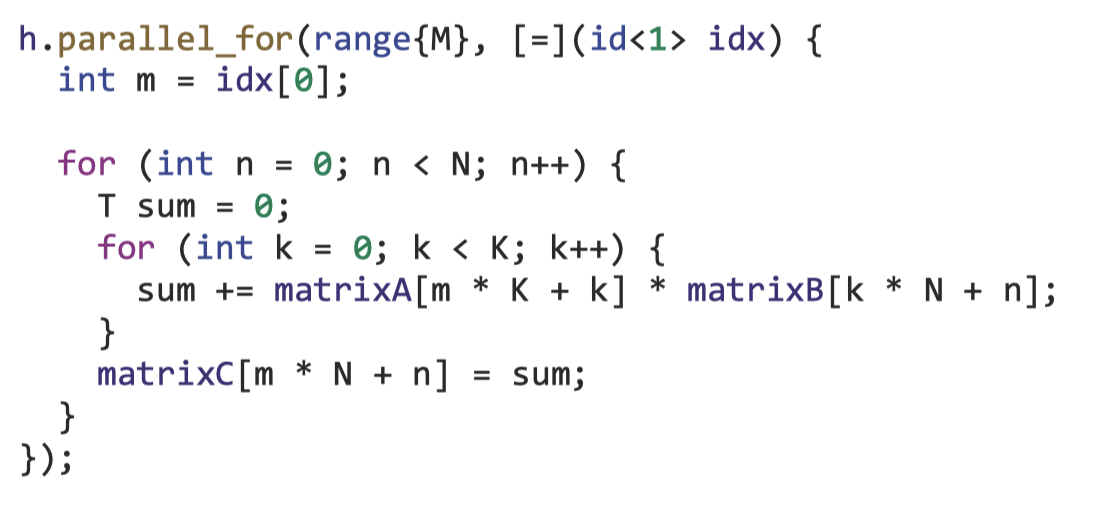
\includegraphics[width=0.9\textwidth]{figs/F15.5.png}
	\caption{\textit{集成电路中的迷宫路由——广度优先搜索的应用:(A) 广度优先搜索,(B) 识别路由路径。}}
\end{figure}

图 15.5 显示了 BFS 在计算机辅助设计(CAD)中的一个重要应用。 在设计集成电路芯片时,需要连接许多电子元件才能完成设计。 
这些组件的连接器称为网络端子。 图15.5(A)以圆点形式示出了两个这样的网络端子; 
一个属于芯片左上部分的组件,另一个属于芯片右下部分的另一个组件。 假设设计要求这两个网络端子相连。 
这是通过将给定宽度的电线从第一网络端子延伸或布线到第二网络端子来完成的。

布线软件将芯片表示为接线块网格,其中每个块都可以充当一根电线。 可以通过沿水平方向或垂直方向延伸来形成线。 
例如,芯片下半部分的黑色J形由21个接线块组成,连接三个网络端子。 
一旦接线块用作电线的一部分,它就不能再用作任何其他电线的一部分。 此外,它还对其周围的接线块形成堵塞。 
没有电线可以从已用块的下邻居延伸到其上邻居,或者从其左邻居延伸到右邻居,依此类推。 
一旦形成电线,所有其他电线都必须围绕它布线。 布线块也可以被电路组件占用,这与用作电线的一部分时施加相同的阻塞约束。 
这就是为什么该问题被称为迷宫路由问题。 先前形成的电路元件和电线为尚未形成的电线形成了迷宫。 
考虑到先前形成的组件和电线的所有约束,迷宫布线软件为每条附加电线找到一条路线。

迷宫路由应用程序将芯片表示为图。 路由块是顶点。 从顶点 $i$ 到顶点 $j$ 的边表示可以将一条线从块 $i$ 延伸到块 $j$。 
一旦某个块被电线或组件占用,它就会被标记为阻塞顶点或从图中删除,具体取决于应用程序的设计。 
图 15.5 显示该应用程序使用 BFS 解决了从根网络终端到目标网络终端的迷宫路由问题。 
这是通过从根顶点开始并将顶点标记为级别来完成的。 不是障碍物的直接垂直或水平邻居(总共四个)被标记为级别 1 。 
我们看到根的所有四个邻居都是可达的,并且将被标记为级别 1 。 当前搜索既不阻塞也不访问的 1 级顶点的邻居将被标记为 2 级。 
读者应该验证图 15.5(A) 中是否有 4 个 1 级顶点、8 个 2 级顶点、12 个 3 级顶点等等。 
正如我们所看到的,BFS 本质上为每个级别形成了一个顶点波前。 这些波前在第 1 级开始时很小,但在几个级别中可以很快变得非常大。

图15.5(B)显示,一旦BFS完成,我们可以通过找到从根到目标的最短路径来形成一条线。 
正如前面所解释的,这可以通过从目标顶点开始并追溯到其级别比当前顶点低一级的前辈来完成。 
每当有多个具有同等级别的前辈时,就会有多条长度相同的路线。 
人们可以设计启发式方法来选择前身,从而最大限度地减少尚未形成的电线的约束难度。

\subsection{广度优先搜索的以顶点为中心的并行化}
并行化图算法的一种自然方法是在不同的顶点或边上并行执行操作。 事实上,图算法的许多并行实现可以分为以顶点为中心或以边为中心。 
以顶点为中心的并行实现将线程分配给顶点,并让每个线程在其顶点上执行操作,这通常涉及迭代该顶点的邻居。 
根据算法的不同,感兴趣的邻居可能是通过传出边缘、传入边缘或两者均可到达的邻居。 
相反,以边为中心的并行实现将线程分配给边,并让每个线程在其边上执行操作,这通常涉及查找该边的源顶点和目标顶点。 
在本节中,我们将研究 BFS 的两种不同的以顶点为中心的并行实现:一种在传出边上迭代,一种在传入边上迭代。 
在下一节中,我们将研究 BFS 的以边缘为中心的并行实现并进行比较。

我们将看到的并行实现在迭代级别时遵循相同的策略。 在所有实现中,我们首先将根顶点标记为属于级别 0 。 
然后,我们调用内核将根顶点的所有邻居标记为属于级别 1 。 之后,我们调用内核将 1 级顶点的所有未访问邻居标记为属于 2 级。 
然后我们调用内核将 2 级顶点的所有未访问邻居标记为属于 3 级。 这个过程一直持续到没有新的顶点被访问和标记为止。

为每个级别调用单独的内核的原因是,我们需要等到上一个级别中的所有顶点都已被标记,然后才能继续标记下一个级别中的顶点。 
否则,我们可能会错误地标记顶点。 在本节的其余部分中,我们重点关注实现每个级别调用的内核。 
也就是说,我们将实现一个 BFS 内核,给定一个级别,根据先前级别的顶点标签来标记属于该级别的所有顶点。

第一个以顶点为中心的并行实现将每个线程分配给一个顶点,以迭代该顶点的传出边缘(Harish 和 Narayanan,2007)。 
每个线程首先检查其顶点是否属于前一层。 如果是这样,线程将遍历传出边缘,将所有未访问的邻居标记为属于当前级别。 
这种以顶点为中心的实现通常称为自顶向下或推送实现。 
\footnote{如果我们正在构建 BFS 树,则此实现可以视为将线程分配给 BFS 树中的父节点以搜索其子节点,因此称为自上而下。 
该术语假设树的根位于顶部,叶子位于底部。 推是指每个活动顶点通过其输出边将其深度推到其所有邻居的操作。}
由于此实现需要可访问给定源顶点的出边(即邻接矩阵的给定行的非零元素),因此需要 CSR 表示。

\begin{figure}[H]
	\centering
	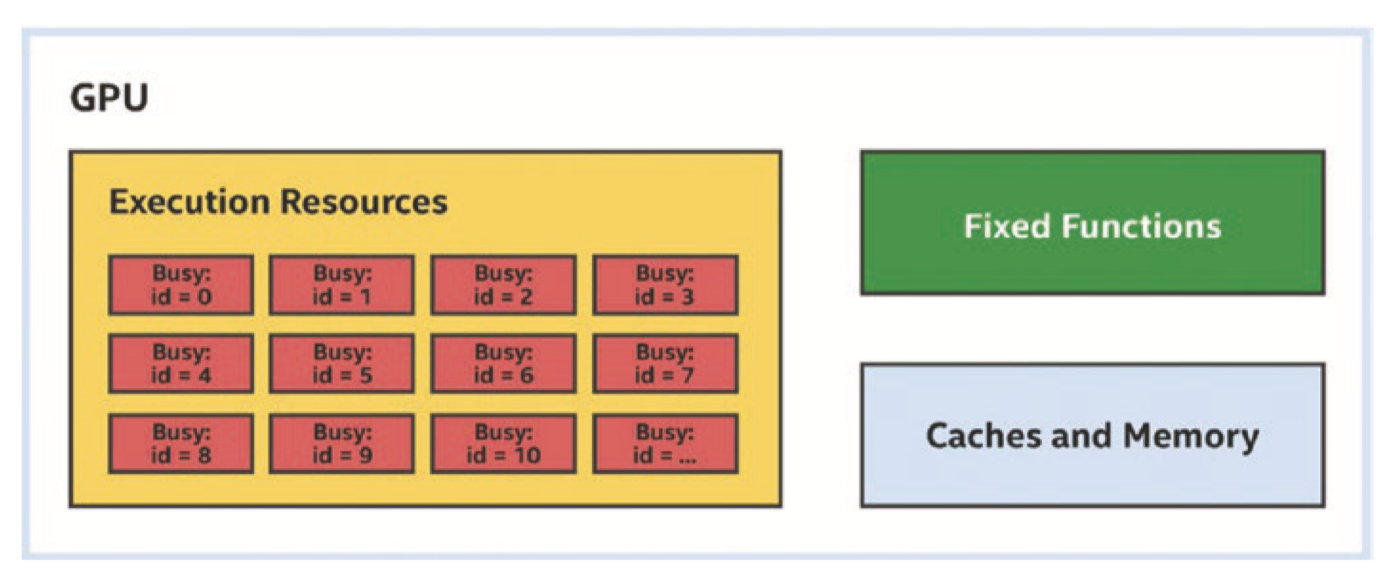
\includegraphics[width=0.9\textwidth]{figs/F15.6.png}
	\caption{\textit{以顶点为中心的推送(自上而下)BFS 内核。 BFS,广度优先搜索。}}
\end{figure}

\begin{figure}[H]
	\centering
	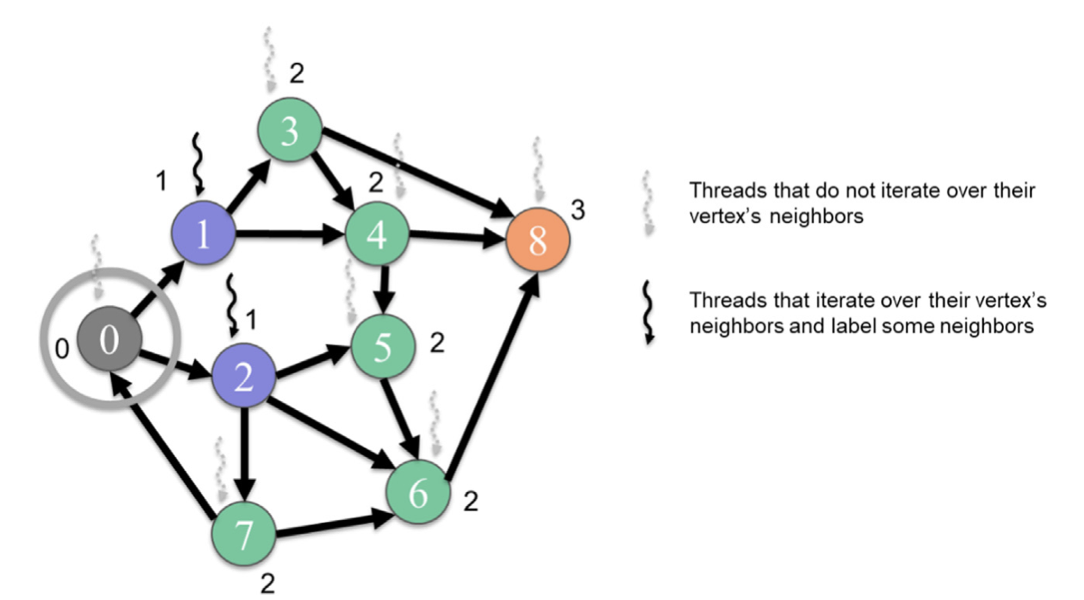
\includegraphics[width=0.9\textwidth]{figs/F15.7.png}
	\caption{\textit{从第 1 层到第 2 层的以顶点为中心的推送 BFS 遍历示例。BFS,广度优先搜索。}}
\end{figure}

图 15.6 显示了以顶点为中心的推送实现的内核代码,
图 15.7 显示了该内核如何执行从级别 1(前一级别)到级别 2(当前级别)的遍历的示例。 
内核首先为每个顶点分配一个线程(第 03 行),并且每个线程确保其顶点 id 在边界内(第 04 行)。 
接下来,每个线程检查其顶点是否属于上一层(第 05 行)。 在图 15.7 中,只有分配给顶点 1 和 2 的线程才会通过此检查。 
然后,通过此检查的线程将使用 CSR srcPtrs 数组来定位顶点的传出边并迭代它们(第 06-07 行)。 
对于每个传出边,线程使用 CSR dst 数组(第 08 行)查找该边的目的地处的邻居。 
然后,该线程通过检查邻居是否已被分配到某个级别来检查邻居是否尚未被访问过(第 09 行)。

最初,所有顶点级别都设置为 UINT\_MAX,这意味着该顶点不可到达。 
因此,如果邻居的级别仍为 UINT\_MAX,则该邻居尚未被访问过。 
如果邻居尚未被访问过,则线程会将邻居标记为属于当前级别(第 10 行)。 
最后,线程将设置一个标志,指示已访问新顶点(第 11 行)。 
启动代码使用此标志来决定是否需要启动新网格来处理新级别,或者我们已经到达终点。 
请注意,多个线程可以将 1 分配给该标志,并且代码仍将正确执行。 该属性称为幂等性。 
在像这样的幂等操作中,我们不需要原子操作,因为线程不执行读取-修改-写入操作。 
所有线程写入相同的值,因此无论有多少线程执行写入操作,结果都是相同的。

第二个以顶点为中心的并行实现将每个线程分配给一个顶点,以迭代该顶点的传入边。 每个线程首先检查其顶点是否已被访问。 
如果不是,线程将迭代传入的边以查找是否有任何邻居属于前一级别。 
如果线程找到属于前一级别的邻居,则线程会将其顶点标记为属于当前级别。 
这种以顶点为中心的实现通常称为自下而上或拉式实现。 
\footnote{如果我们正在构建 BFS 树,则此实现可以视为将线程分配给 BFS 树中的潜在子节点以搜索其父节点,因此称为自下而上。 
拉动是指每个顶点返回其前任顶点并从中拉出活动状态的动作。}
由于此实现需要可访问给定目标顶点的传入边(即邻接矩阵的给定列的非零元素),因此需要 CSC 表示。

\begin{figure}[H]
	\centering
	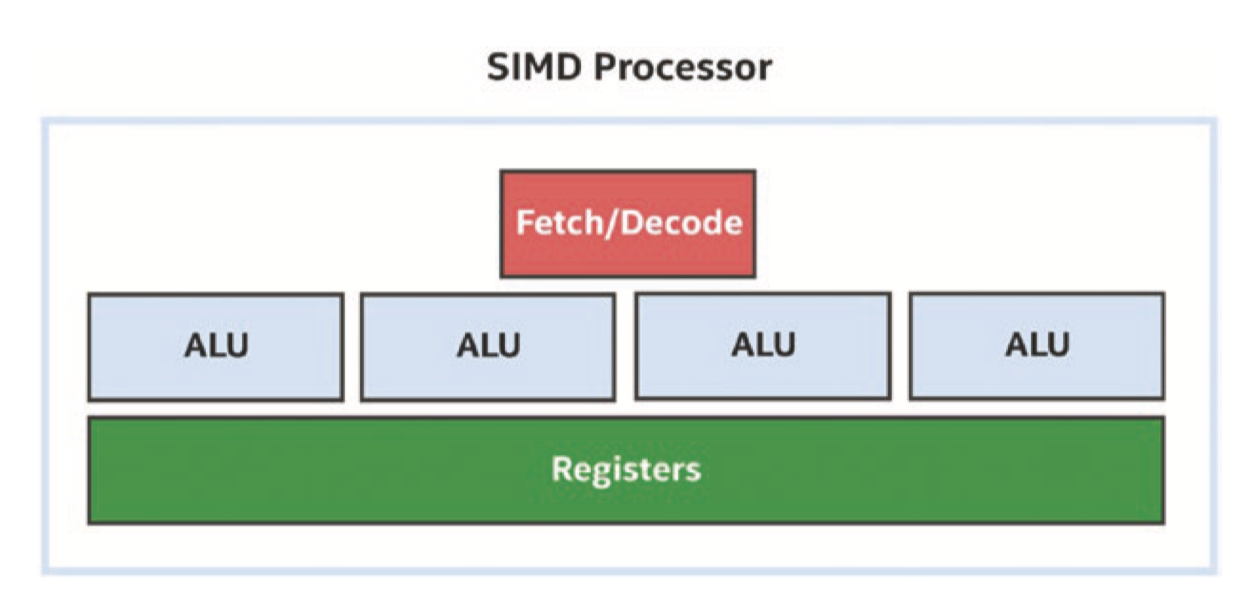
\includegraphics[width=0.9\textwidth]{figs/F15.8.png}
	\caption{\textit{以顶点为中心的拉式(自下而上)BFS 内核。 BFS,广度优先搜索。}}
\end{figure}

图 15.8 显示了以顶点为中心的拉实现的内核代码,图 15.9 显示了该内核如何执行从级别 1 到级别 2 的遍历的示例。 
内核首先为每个顶点分配一个线程(第 03 行),并且每个线程确保其顶点 id 在边界内(第 04 行)。 
接下来,每个线程检查其顶点是否尚未被访问(第 05 行)。 在图 15.9 中,分配给顶点 3-8 的线程都通过了此检查。 
然后,通过此检查的线程将使用 CSC dstPtrs 数组来定位顶点的传入边并迭代它们(第 06-07 行)。 
对于每个传入边,线程使用 CSC src 数组(第 08 行)查找边源处的邻居。 然后该线程检查邻居是否属于前一层(第 09 行)。 
如果是这样,线程会将其顶点标记为属于当前级别(第 10 行),并设置一个标志来指示已访问新顶点(第 11 行)。 
该线程也将跳出循环(第 12 行)。

\begin{figure}[H]
	\centering
	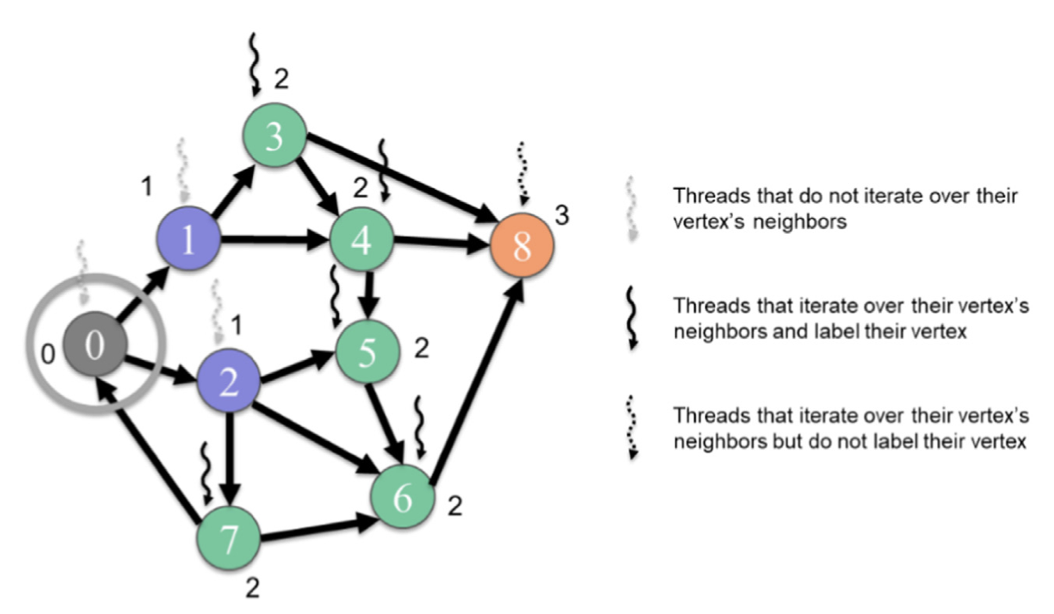
\includegraphics[width=0.9\textwidth]{figs/F15.9.png}
	\caption{\textit{从级别 1 到级别 2 以顶点为中心的拉动(自下而上)遍历的示例。}}
\end{figure}

跳出循环的理由如下。 对于要确定其顶点位于当前级别的线程,该线程的顶点在前一级别中有一个邻居就足够了。 
因此线程没有必要检查其余的邻居。 只有其顶点在前一层中没有任何邻居的线程才会最终循环遍历整个邻居列表。 
在图 15.9 中,只有分配给顶点 8 的线程才会在整个邻居列表上循环而不会中断。

在比较以顶点为中心的推式和拉式并行实现时,需要考虑两个对性能有重要影响的关键差异。 
第一个区别是,在推实现中,线程在其顶点的整个邻居列表上循环,而在拉实现中,线程可能会提前脱离循环。 
对于低度和低方差的图(例如道路网络或 CAD 电路模型),这种差异可能并不重要,因为邻居列表很小且大小相似。 
然而,对于具有高度数和高方差的图(例如社交网络),邻居列表很长并且大小可能变化很大,导致线程间的负载不平衡和控制发散。 
因此,尽早跳出循环可以通过减少负载不平衡和控制发散来提供显着的性能增益。

两种实现之间的第二个重要区别是,在推实现中,只有分配给前一级别中的顶点的线程在其邻居列表上循环,
而在拉实现中,分配给任何未访问顶点的所有线程在其邻居列表上循环 。 
对于早期级别,我们预计每个级别的顶点数量相对较少,而图中有大量未访问的顶点。 
因此,推送实现通常对于较早的级别表现更好,因为它迭代的邻居列表较少。 
相反,对于后面的级别,我们期望每个级别有更多的顶点,并且图中未访问的顶点更少。 
此外,在拉式方法中找到访问过的邻居并提前退出循环的机会更高。 因此,拉式实现通常在后面的级别上表现更好。

根据这一观察,常见的优化是对较早的级别使用推送实现,然后在后面的级别切换到拉取实现。 这种方法通常被称为方向优化实现。 
何时在实现之间切换的选择通常取决于图的类型。 
低度图通常具有许多级别,并且需要一段时间才能达到级别具有许多顶点并且大量顶点已被访问的点。 
另一方面,高度图通常层次很少,而且层次增长非常快。 从任意顶点到任意其他顶点只需要几个层的高阶图通常被称为小世界图。 
由于这些属性,对于高度图,从推实现切换到拉实现通常比低度图早得多。

回想一下,推送实现使用图的 CSR 表示,而拉实现使用图的 CSC 表示。 
因此,如果要使用方向优化实现,则需要存储图的 CSR 和 CSC 表示。 
在许多应用中,例如社交网络或迷宫路由,图是无向的,这意味着邻接矩阵是对称的。 
在这种情况下,CSR 和 CSC 表示形式是等效的,因此只需要存储其中之一,并且两种实现都可以使用它们。

\subsection{广度优先搜索的以边缘为中心的并行化}
在本节中,我们将研究 BFS 的以边缘为中心的并行实现。 
在此实现中,每个线程都分配给一条边。 它检查边的源顶点是否属于前一层以及边的目标顶点是否未被访问。 
如果是,它将未访问的目标顶点标记为属于当前级别。 
由于此实现需要可访问给定边的源顶点和目标顶点(即给定非零的行索引和列索引),因此需要 COO 数据结构。

\begin{figure}[H]
	\centering
	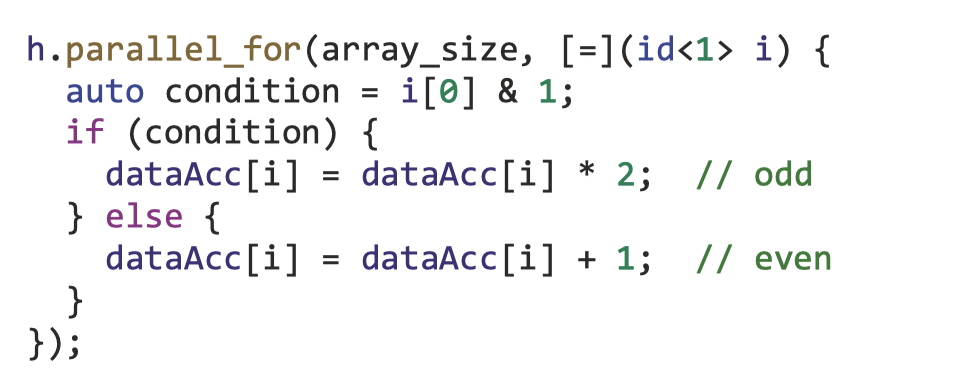
\includegraphics[width=0.9\textwidth]{figs/F15.10.png}
	\caption{\textit{以边缘为中心的 BFS 内核。 BFS,广度优先搜索。}}
\end{figure}

\begin{figure}[H]
	\centering
	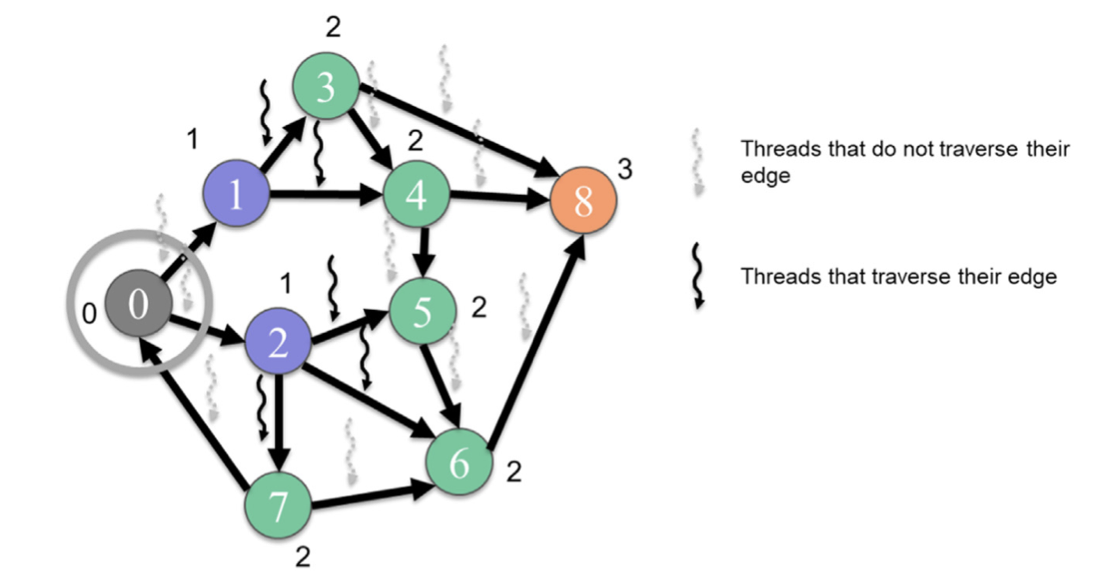
\includegraphics[width=0.9\textwidth]{figs/F15.11.png}
	\caption{\textit{从级别 1 到级别 2 以边为中心的遍历的示例。}}
\end{figure}

图 15.10 显示了以边为中心的并行实现的内核代码,而图 15.11 显示了该内核如何执行从级别 1 到级别 2 的遍历的示例。
内核首先为每个边分配一个线程(第 03 行) ,并且每个线程确保其边缘 id 在边界内(第 04 行)。 
接下来,每个线程使用 COO src 数组查找其边的源顶点(第 05 行),并检查该顶点是否属于上一层(第 06 行)。 
在图 15.11 中,只有分配给顶点 1 和 2 的出边的线程才会通过此检查。 
通过此检查的线程将使用 COO dst 数组(第 07 行)将邻居定位在边缘的目的地,并检查邻居是否尚未被访问(第 08 行)。 
如果不是,线程会将邻居标记为属于当前级别(第 09 行)。 最后,线程将设置一个标志,指示已访问新顶点(第 10 行)。

与以顶点为中心的并行实现相比,以边为中心的并行实现有两个主要优点。 第一个优点是以边缘为中心的实现展示了更多的并行性。 
在以顶点为中心的实现中,如果顶点数量很少,我们可能无法启动足够的线程来完全占用设备。 
由于图的边通常比顶点多得多,因此以边为中心的实现可以启动更多线程。 因此,以边缘为中心的实现通常更适合小图。

与以顶点为中心的实现相比,以边缘为中心的实现的第二个优点是它表现出更少的负载不平衡和控制发散。 
在以顶点为中心的实现中,每个线程迭代不同数量的边,具体取决于分配给它的顶点的度数。 
相反,在以边为中心的实现中,每个线程仅遍历一条边。 
对于以顶点为中心的实现,以边为中心的实现是重新安排线程到工作或数据的映射以减少控制分歧的示例,
如第 6 章“性能注意事项”中所述。 以边为中心的实现通常更适合顶点度数变化较大的高度图。

以边为中心的实现的缺点是它会检查图中的每条边。 相反,如果实现确定顶点与级别不相关,则以顶点为中心的实现可以跳过整个边列表。 
例如,考虑某些顶点 $v$ 具有 $n$ 边并且与特定级别不相关的情况。 
在以边缘为中心的实现中,我们的启动包括 $n$ 个线程,每个边缘一个线程,每个线程独立检查 $v$ 并发现边缘不相关。 
相比之下,在以顶点为中心的实现中,我们的启动仅包含 $v$ 的一个线程,该线程在检查 $v$ 一次以确定其不相关后跳过所有 $n$ 边。 
以边为中心的实现的另一个缺点是它使用 $\mathrm{COO}$,与以顶点为中心的实现使用的 CSR 和 CSC 相比,
它需要更多的存储空间来存储边。

读者可能已经注意到,上一节和本节中的代码示例类似于第 14 章“稀疏矩阵计算”中稀疏矩阵向量乘法 (SpMV) 的实现。 
事实上,通过稍微不同的公式,我们可以完全用 SpMV 和一些其他向量运算来表达 BFS 级别迭代,其中 SpMV 运算是主要运算。 
除了 BFS 之外,许多其他图计算也可以使用邻接矩阵根据稀疏矩阵计算来制定(Jeremy 和 Gilbert,2011)。 
这样的公式通常被称为图问题的线性代数公式,并且是称为 GraphBLAS 的 API 规范的焦点。 
线性代数公式的优点是它们可以利用成熟且高度优化的稀疏线性代数并行库来执行图计算。 
线性代数公式的缺点是它们可能会错过利用相关图算法的特定属性的优化。

\subsection{提高边界效率}
在前两节讨论的方法中,我们检查每次迭代中的每个顶点或边与所讨论级别的相关性。 
这种策略的优点是内核是高度并行的并且不需要跨线程的任何同步。 缺点是启动了许多不必要的线程并执行了大量无用的工作。 
例如,在以顶点为中心的实现中,我们为图中的每个顶点启动一个线程,其中许多线程只是发现该顶点不相关并且不执行任何工作。 
类似地,在以边为中心的实现中,我们为图中的每个边启动一个线程; 许多线程只是发现边缘不相关并且不执行任何有用的工作。

在本节中,我们的目标是避免启动不必要的线程并消除它们在每次迭代中执行的冗余检查。 
我们将重点关注第 15.3 节中介绍的以顶点为中心的推送方法。 
回想一下,在以顶点为中心的推送方法中,对于每个级别,都会为图中的每个顶点启动一个线程。 
该线程检查其顶点是否位于上一层,如果是,则将该顶点的所有未访问邻居标记为属于当前层。 
另一方面,顶点不在当前层的线程不执行任何操作。 理想情况下,这些线程甚至不应该启动。 
为了避免启动这些线程,我们可以让处理前一级别中的顶点的线程协作构建它们访问的顶点的边界。 
因此,对于当前级别,仅需要为该边界中的顶点启动线程(Luo et al., 2010)。

\begin{figure}[H]
	\centering
	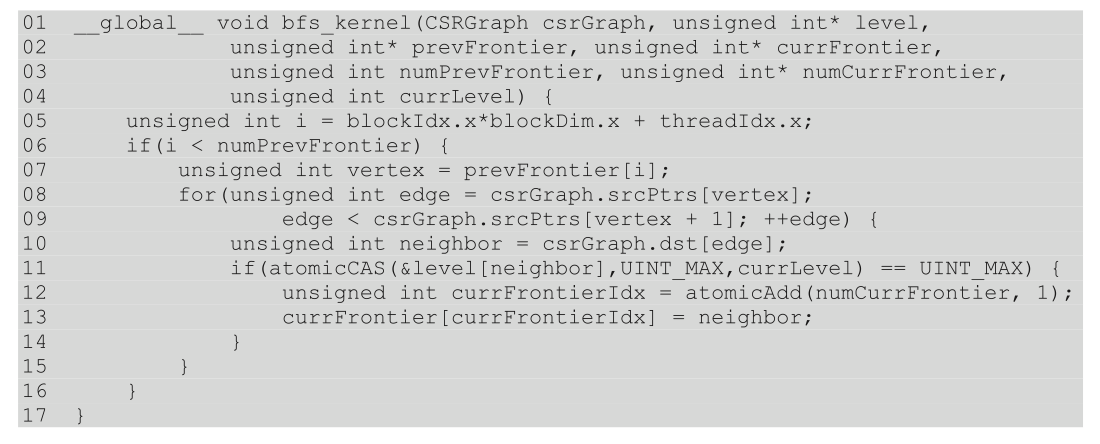
\includegraphics[width=0.9\textwidth]{figs/F15.12.png}
	\caption{\textit{具有边界的以顶点为中心的推送(自上而下)BFS 内核。 BFS,广度优先搜索。}}
\end{figure}

\begin{figure}[H]
	\centering
	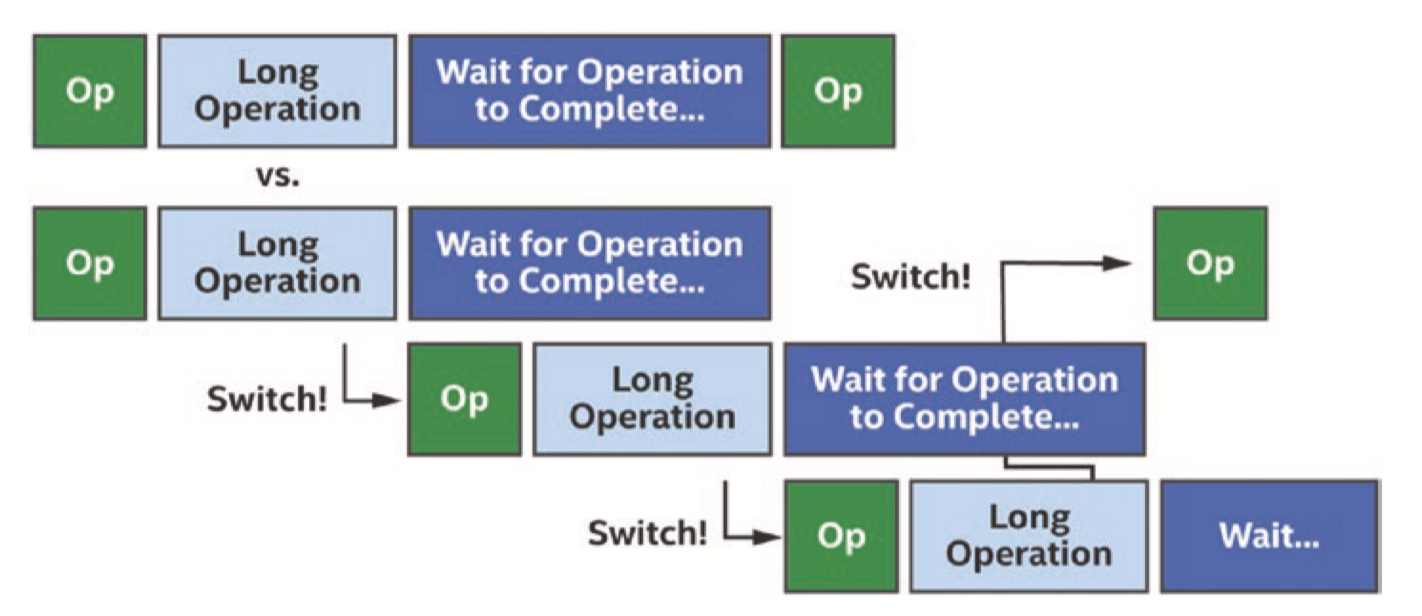
\includegraphics[width=0.9\textwidth]{figs/F15.13.png}
	\caption{\textit{以顶点为中心的推(自上而下)BFS 遍历从级别 1 到级别 2(带边界)的示例。 BFS,广度优先搜索。}}
\end{figure}

图 15.12 显示了使用边界的以顶点为中心的推送实现的内核代码,图 15.13 显示了该内核如何执行从级别 1 到级别 2 的遍历的示例。
与之前方法的一个关键区别是,内核 采用附加参数来表示边界。 
附加参数包括数组 prevfrontier 和 currfrontier,分别用于存储先前边界和当前边界中的顶点。 
它们还包括指向计数器 numprevFrontier 和 numCurrfrontier 的指针,这些计数器存储每个边界中的顶点数。 
请注意,不再需要用于指示已访问新顶点的标志。 相反,当当前边界中的顶点数为 0 时,主机可以判断已到达终点。

现在我们看看图 15.12 中的内核主体。 
内核首先为前一个边界的每个元素分配一个线程(第 05 行),并且每个线程确保其元素 id 在边界内(第 06 行)。 
在图15.13中,只有顶点1和2位于前一个边界中,因此只启动了两个线程。 
每个线程从前一个边界加载其元素,其中包含它正在处理的顶点的索引(第 07 行)。 
该线程使用 CSR srcPtrs 数组来定位顶点的传出边并迭代它们(第 08-09 行)。 
对于每个传出边,线程使用 CSR dst 数组(第 10 行)查找该边的目的地处的邻居。 然后该线程检查邻居是否还没有被访问过; 
如果不是,则将邻居标记为属于当前级别(第 11 行)。 与之前的实现的一个重要区别是,使用原子操作来执行检查和标记操作。 
稍后将解释原因。 如果线程成功标记邻居,它必须将邻居添加到当前边界。 
为此,线程增加当前边界的大小(第 12 行)并将邻居添加到相应的位置(第 13 行)。 
当前边界的大小需要以原子方式递增(第 12 行),因为多个线程可能会同时递增它,因此我们需要确保不会发生竞争条件。

现在我们将注意力转向第 11 行的原子操作。当线程迭代其顶点的邻居时,它会检查邻居是否已被访问; 
如果不是,则将邻居标记为属于当前级别。 
在图 15.12 中的无边界的以顶点为中心的推送内核中,这种检查和标记操作是在没有原子操作的情况下执行的(09-10)。 
在该实现中,如果多个线程在它们中的任何一个能够标记它之前检查同一个未访问的邻居的旧标签,则多个线程最终可能会标记该邻居。 
由于所有线程都使用相同的标签来标记邻居(该操作是幂等的),因此允许线程冗余地标记邻居是可以的。 
相比之下,在图 15.12 中基于边界的实现中,每个线程不仅标记未访问的邻居,而且还将其添加到边界。 
因此,如果多个线程观察到邻居未被访问,它们都会将邻居添加到边界,从而导致它被多次添加。 
如果多次将邻居添加到边界中,则在下一级中将对其进行多次处理,这是冗余和浪费的。 
为了避免多个线程将邻居视为未访问,应以原子方式执行邻居标签的检查和更新。 
换句话说,我们必须检查邻居是否未被访问过,如果没有,则将其标记为当前级别的一部分,所有这一切都在一个原子操作中完成。 
可以执行所有这些步骤的原子操作是比较和交换,它由atomicCAS 内部函数提供。 
该函数采用三个参数:内存中数据的地址、我们要与数据进行比较的值以及如果比较成功,我们要将数据设置为的值。 
在我们的例子中(第 11 行),我们希望将 1eve][neighbor] 与 UINT\_MAX 进行比较,以检查邻居是否未被访问,
如果比较成功,则将 level[neighbor] 设置为 currLevel。 与其他原子操作一样,atomicCAS 返回所存储数据的旧值。 
因此,我们可以通过将atomicCAS的返回值与atomicCAS所比较的值(在本例中为UINT\_MAX)进行比较来检查compareand-swap操作是否成功。

如前所述,这种基于边界的方法相对于上一节中描述的方法的优点在于,它仅通过启动线程来处理相关顶点来减少冗余工作。 
这种基于边界的方法的缺点是长延迟原子操作的开销,特别是当这些操作争用相同的数据时。 
对于atomicCAS操作(第11行),我们期望争用是适度的,因为只有一些线程(而不是全部)会访问同一个未访问的邻居。 
然而,对于atomicAdd操作(第12行),我们预计争用会很高,因为所有线程都会增加相同的计数器以将顶点添加到相同的边界。 
在下一节中,我们将探讨如何减少这种争用。

\subsection{通过私有化减少争用}
回想一下第 6 章“性能注意事项”,可用于减少对同一数据的原子操作争用的一种优化是私有化。 
私有化通过对数据的私有副本应用部分更新,然后在完成后更新公共副本来减少原子争用。 
我们在第 9 章“并行直方图”中看到了直方图模式私有化的示例,
其中同一块中的线程更新了该块私有的局部直方图,然后在最后更新了公共直方图。

私有化也可以应用于并发前沿更新(numcurrfrontier 的增量)的上下文中,以减少插入前沿时的争用。 
我们可以让每个线程块在整个计算过程中维护自己的局部边界,并在完成后更新公共边界。 
因此,线程只会与同一块中的其他线程竞争相同的数据。 
此外,局部边界及其计数器可以存储在共享内存中,这使得可以对计数器进行低延迟的原子操作并将其存储到局部边界。 
此外,当共享内存中的局部边界存储到全局内存中的公共边界时,可以合并访问。

\begin{figure}[H]
	\centering
	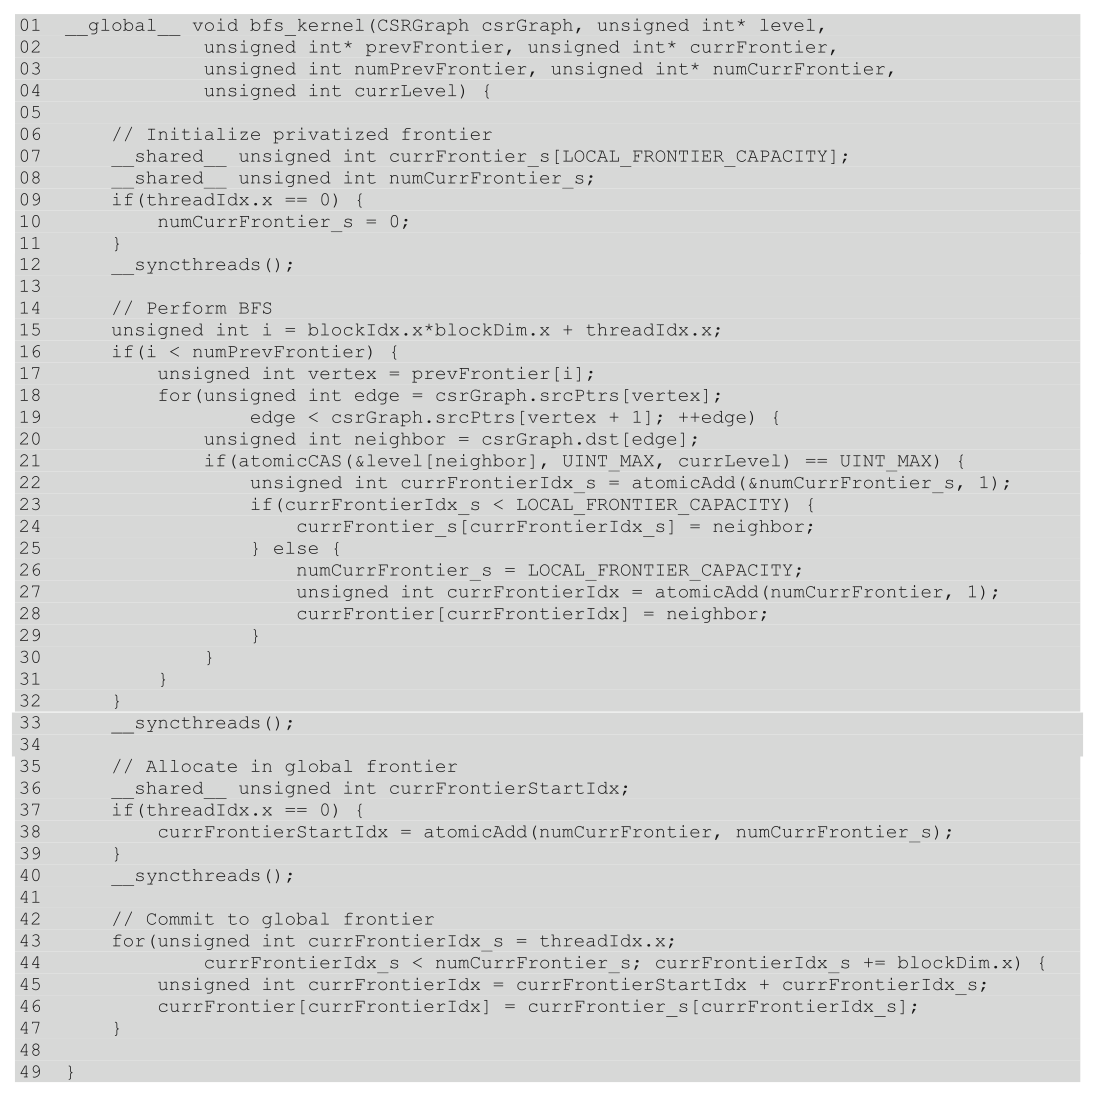
\includegraphics[width=0.9\textwidth]{figs/F15.14.png}
	\caption{\textit{具有边界私有化的以顶点为中心的推送(自上而下)BFS 内核。 BFS,广度优先搜索。}}
\end{figure}

\begin{figure}[H]
	\centering
	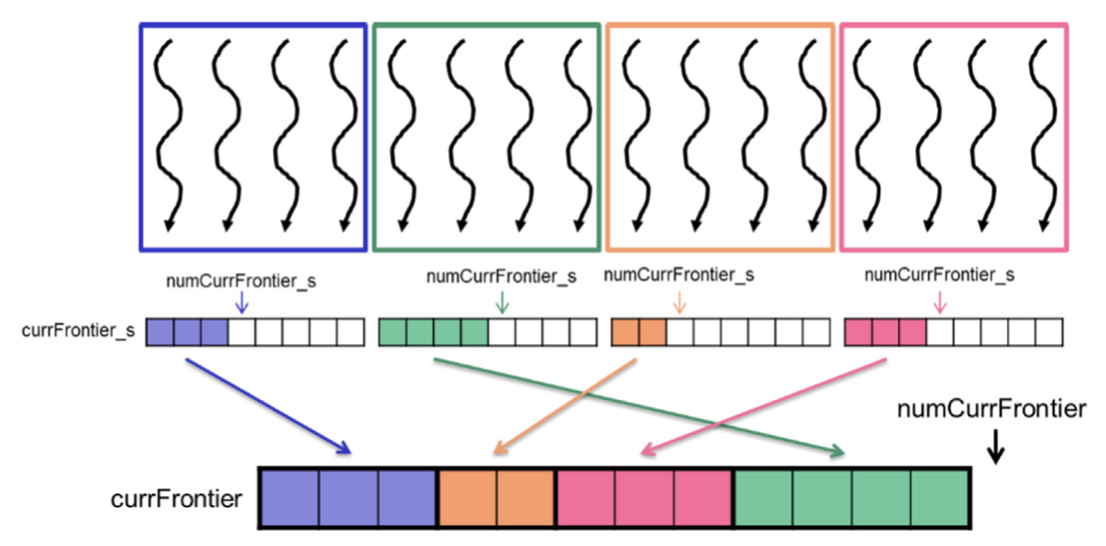
\includegraphics[width=0.9\textwidth]{figs/F15.15.png}
	\caption{\textit{边界私有化的例子。}}
\end{figure}

图 15.14 显示了使用私有化前沿的以顶点为中心的推送实现的内核代码,而图 15.15 说明了前沿的私有化。 
内核首先为共享内存中的每个线程块声明一个私有边界(第 07-08 行)。 
块中的一个线程将前沿计数器初始化为 0(第 09-11 行),
块中的所有线程在开始使用计数器之前在 \_syncthreads 屏障处等待初始化完成(第 12 行)。 
代码的下一部分与之前的版本类似:每个线程从边界加载其顶点(第 17 行),
迭代其传出边(第 18-19 行),在边的目的地查找邻居(第 20 行) ),
并自动检查邻居是否未被访问,如果未被访问则访问它(第 21 行)。

如果线程成功访问邻居,即邻居未被访问,则将邻居添加到局部边界。 线程首先以原子方式递增局部边界计数器(第 22 行)。 
如果局部边界未满(第 23 行),则线程将邻居添加到局部边界(第 24 行)。 
否则,如果局部边界已溢出,则线程恢复局部计数器的值(第 26 行),
并通过自动递增全局计数器(第 27 行)并将邻居存储在相应位置(第 27 行)来将邻居添加到全局边界中。 28)。

在块中的所有线程迭代其顶点的邻居之后,它们需要将私有化的局部边界存储到全局边界。 
首先,线程等待彼此完成,以确保不会有更多的邻居被添加到局部边界(第 33 行)。 
接下来,块中的一个线程代表其他线程在全局边界中为局部边界中的所有元素分配空间(第 36-39 行),
同时所有线程都等待它(第 40 行)。 
最后,线程迭代局部边界中的顶点(第 43-44 行)并将它们存储在公共边界中(第 45-46 行)。 
请注意,公共前沿 currfrontierIdx 的索引以 currfrontierIdx\_s 表示,而 currfrontierIdx\_s 以 threadIdx.x 表示。 
因此,具有连续线程索引值的线程存储到连续的全局内存位置,这意味着存储是合并的。

\subsection{其他优化}
\subsubsection{减少启动开销}
在大多数图中,BFS 初始迭代的边界可能非常小。 第一次迭代的边界只有源的邻居。 
下一次迭代的边界具有当前边界顶点的所有未访问的邻居。 在某些情况下,最后几次迭代的边界也可能很小。 
对于这些迭代,终止网格和启动新网格的开销可能超过并行性的好处。 
处理这些小边界迭代的一种方法是准备另一个仅使用一个线程块但可以执行多个连续迭代的内核。 
内核仅使用局部块级边界,并使用 \_\_syncthreads ( ) 来同步级别之间的所有线程。

\begin{figure}[H]
	\centering
	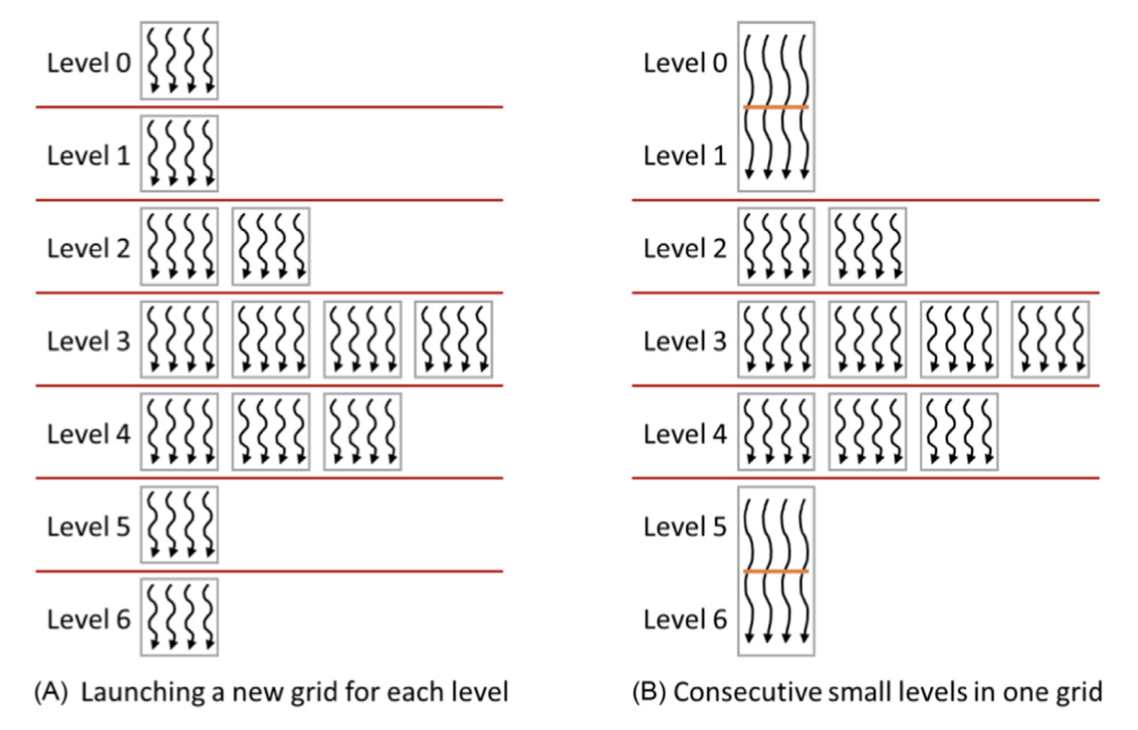
\includegraphics[width=0.9\textwidth]{figs/F15.16.png}
	\caption{\textit{对于具有小边界的级别在一个网格中执行多个级别:(A) 为每个级别启动一个新网格,
	(B) 在一个网格中连续的小级别。}}
\end{figure}

这种优化如图 15.16 所示。 在此示例中,级别 0 和级别 1 均可由单个线程块处理。 
我们没有为级别 0 和 1 启动单独的网格,而是启动单块网格并使用 \_\_syncthreads ( ) 在级别之间进行同步。 
一旦边界达到溢出块级边界的大小,块中的线程就会将块级边界内容复制到全局边界并返回到主机代码。 
然后,主机代码将在后续级别迭代中调用常规内核,直到边界再次变小。 
因此,单块内核消除了小边界迭代的启动开销。 我们将其实现留给读者作为练习。

\subsubsection{改善负载平衡}
回想一下,在以顶点为中心的实现中,每个线程要完成的工作量取决于分配给它的顶点的连接性。 
在某些图中,例如社交网络图中,某些顶点(名人)的度数可能比其他顶点的度数高几个数量级。 
发生这种情况时,一个或几个线程可能会花费过长的时间并减慢整个网格的执行速度。 
我们已经找到了解决这个问题的一种方法,那就是使用以边缘为中心的并行实现。 
我们可以解决此问题的另一种方法是根据边界的度数将边界顶点分类到桶中,并使用适当大小的处理器组在单独的内核中处理每个桶。 
一种值得注意的实现(Merrill 和 Garland,2012)对具有小、中和大度数的顶点使用三种不同的存储桶。 
处理小桶的内核将每个顶点分配给单个线程; 处理中型桶的内核将每个顶点分配给单个warp; 
处理大桶的内核将每个顶点分配给整个线程块。 此技术对于顶点度数变化较大的图特别有用。

\subsubsection{进一步的挑战}
虽然 BFS 是最简单的图应用程序之一,但它呈现出更复杂应用程序特有的挑战:
提取并行性的问题分解、利用私有化、实现细粒度负载平衡以及确保正确的同步。 
图计算适用于各种有趣的问题,特别是在提出建议、检测社区、查找图中的模式以及识别异常等领域。 
一项重大挑战是处理大小超过 GPU 内存容量的图。 
另一个有趣的机会是在开始计算之前将图预处理为其他格式,以便暴露更多并行性或局部性或促进负载平衡。

\subsection{总结}
在本章中,我们以广度优先搜索为例,了解了与并行图计算相关的挑战。 我们首先简要介绍了图的表示。 
我们讨论了以顶点为中心和以边为中心的并行实现之间的差异,并观察了它们之间的权衡。 
我们还看到了如何通过利用边界来消除冗余工作,并通过私有化来优化边界的使用。 
我们还简要讨论了其他高级优化,以减少同步开销并改善负载平衡。